\documentclass[solution, letterpaper]{cs121}

\usepackage{tikz-qtree}
\usepackage{graphicx}

%% Please fill in your name and collaboration statement here.
%\newcommand{\studentName}{Renzo Lucioni and Daniel Broudy}
%\newcommand{\collaborationStatement}{I collaborated with...}
\newcommand{\solncolor}{red}
\begin{document}

\header{X}{May 9, 2013, at 23:59}{}{}

%%%%%%%%%%%%%%%%%%%%%%%%%%%%%%%%%%%%%%%%%%%%%%%%%%%%

\section*{Overview}
\hspace{4mm} To implement our player for the final project, we chose to use an artificial neural network, a finite memory policy, and Q-learning. The following writeup describes the motivation behind using each of these methods, explains the design of each method, discusses the application of each method in the context of playing the game, and then evaluates the performance of each method. 

\section{Artificial Neural Network}
\subsection{Motivation}
\hspace{4mm} When our player requests a plant observation, it receives a noisy image. The player must be able to decide what kind of plant, nutritious or poisonous, is depicted in the image. In order to give our player this capability, we trained a neural network on labeled images. As we learned in Homework 2, a multi-layer feed-forward neural network is a good approach to image classification, superior to decision trees, boosted decision stumps, and perceptrons. 

Like perceptrons, multi-layer feed-forward neural networks are capable of making use of all pixels in an image, allowing them to learn the relationships between pixels. However, unlike perceptrons, neural networks can also use hidden layers to recognize non-linearly separable functions. This allows neural networks to recognize rotations, translations, and skews (i.e., noise) that would have defeated a perceptron. Thus, neural networks are both accurate and robust when determining the class of an input image, whether it be a digit or a plant.

\subsection{Design}
\hspace{4mm} We extracted images using the default players provided to us which always consume a plant if one is present. By ``extract," we mean we wrote requested images to a file. We determined labels for these stored images by calculating the difference in life points before and after eating the plant. A difference greater than 10 meant the plant consumed previously was nutritious, and a difference less than -10 meant that that plant consumed previously was poisonous. We then processed the data by assigning labels to each image and formatting it in a way conducive to being used to train a neural network.

We modified our neural network code from Homework 2 to train on $6 \times 6$ images. We also modified the parser to allow our neural network to handle images as they are provided, as 36 element tuples. LIST OTHER CHANGES

\subsection{Application}
\hspace{4mm} The neural network we trained for this component of the game is able to distinguish between the two kinds of plant images. Our player uses the neural network's output to help it decide what kind of plant it is looking at.

There are 5410 poisonous images and 5590 nutritious images in our collection of 11000 images.

\subsection{Evaluation}
\begin{center}
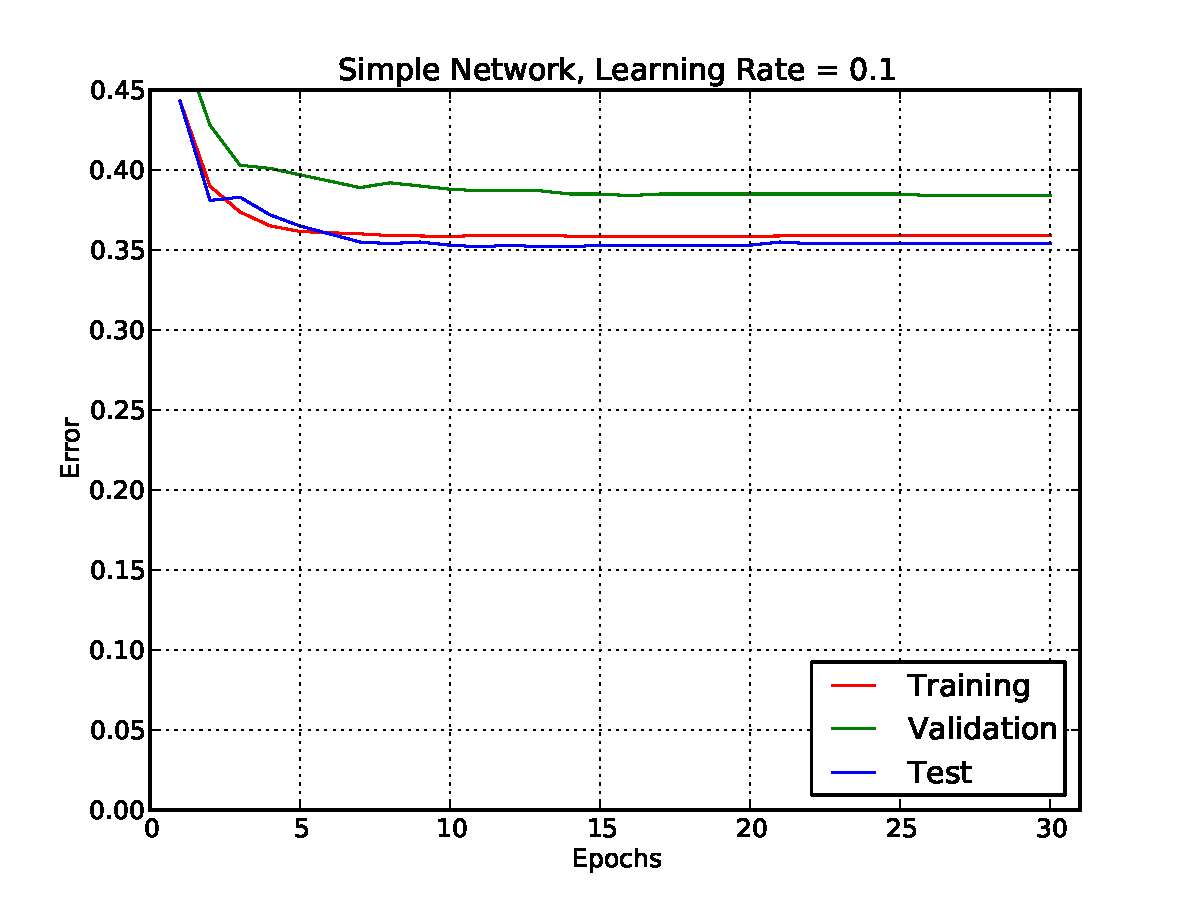
\includegraphics[scale=0.8]{source/simple-network-alpha-0_1.pdf}
\end{center}

In order to test the performance of our player, we first made some slight changes to the handout code to make it run faster and to prevent the game from hanging on enter at the end of the game. These changes required removing calls to {\tt sleep} and {\tt sys.stdin.read(1)}. We then used our {\tt win\_loss\_ratio} script, called with the number of games you want to run as an argument (e.g., 100). This gave us a more objective measure of performance that running the game a handful of times.

\section{Finite Memory Policy}
\subsection{Motivation}
\hspace{4mm} Our neural network does not have error of 0 when classifying images. However, as described above, our ANN classifies images incorrectly with probability X (test error), and the probability of the neural network classifying a plant incorrectly two times in a row is low ($X^2$). This is where a finite memory policy becomes useful.

\subsection{Design}

(Note that we also implemented a finite state controller policy, but decided that the finite memory policy was better because it required fewer observations to make a decision on a plant's type.)
\subsection{Application}
\subsection{Evaluation}
%It's actually not that good because our ANN makes a classification decision regardless of noise. So requesting an observation multiple times is a waste of life points. 

\section{Q-Learning}
\subsection{Motivation}
We want to know how to make the best movement decision (i.e., action) based on our current position in the world (i.e., state). We defined 4 states, each depending on what happened in the last round. Our states are {\sc passed}, {\sc ate nutritious}, {\sc ate poisonous}, and {\sc seen nothing}.

\subsection{Design}
We ran experiments to collect data on the distribution of plants. We did this by running both random, base players and recording their location every time a plant was encountered (i.e., {\tt hasPlant} was set to true). We determined the kind of plant at each location in the same way as we determined labels for the plant images, by looking at the difference in life points before and after eating the plant. For convenience, we set the plant bonus to 1, the plant penalty to 1, the starting life to 100, and the observation cost and life per turn to 0. Below are plots showing the location of nutritious plants (blue dots) and poisonous plants (red dots) in the world. The third plot shows the plot of the nutritious plants superimposed on the plot of the poisonous plants.

\begin{center}
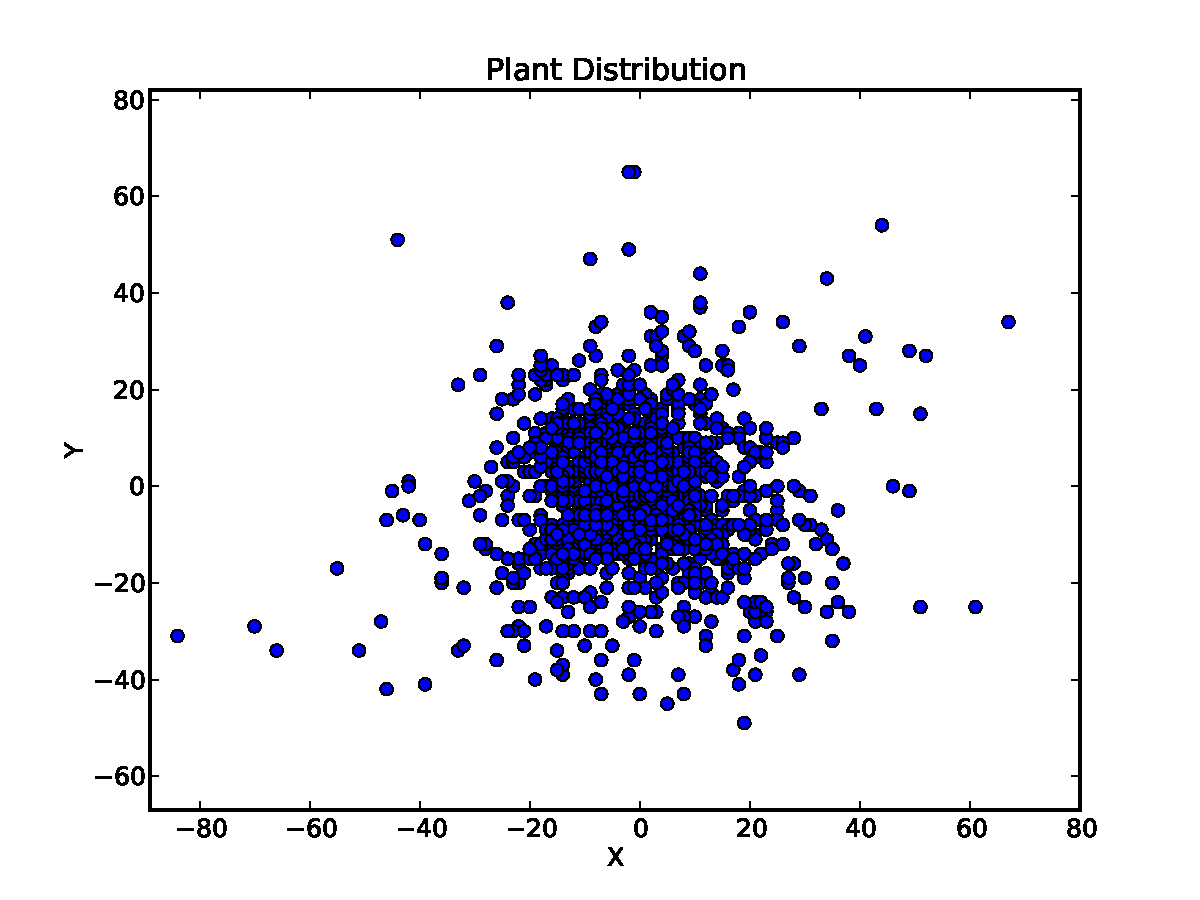
\includegraphics[scale=0.8]{source/nutritious-plant-distribution.pdf}
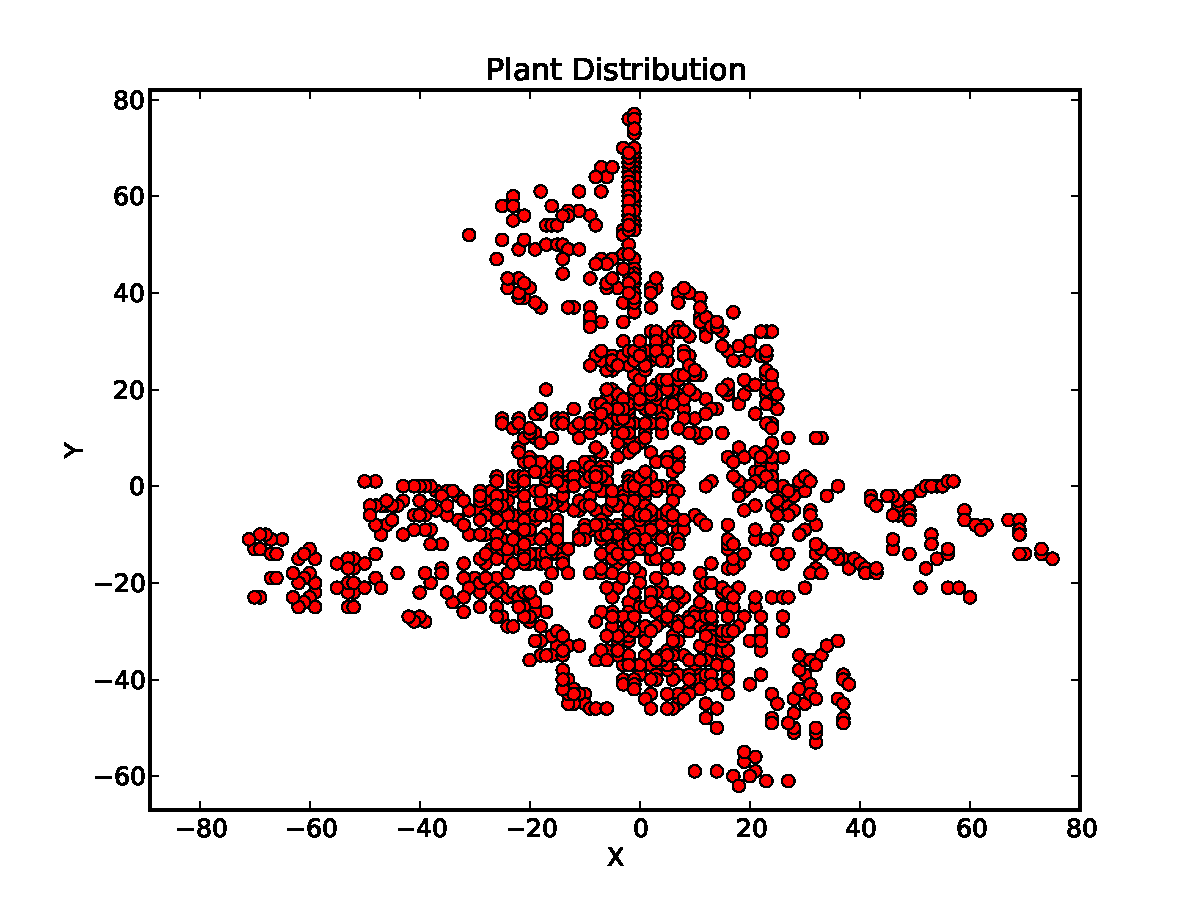
\includegraphics[scale=0.8]{source/poisonous-plant-distribution.pdf}
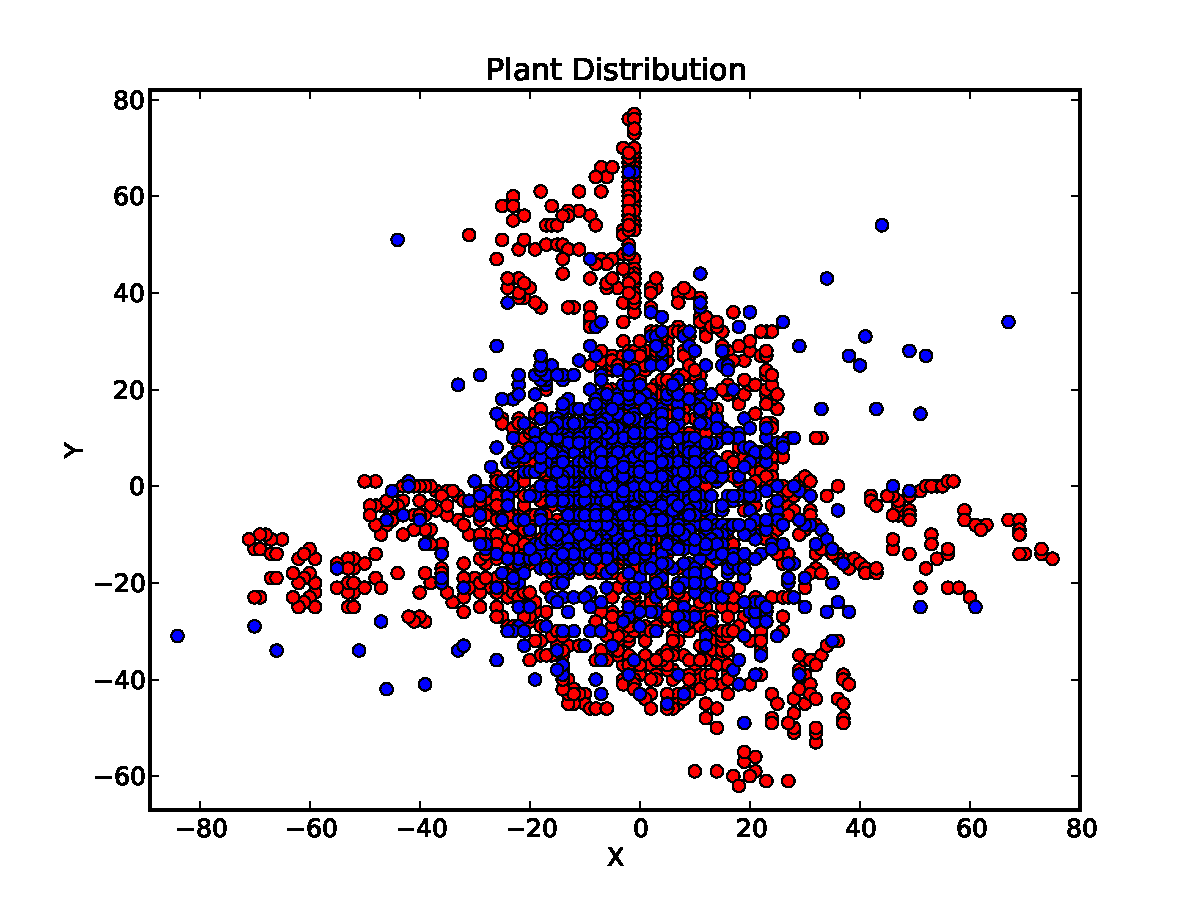
\includegraphics[scale=0.8]{source/plant-distribution.pdf}
\end{center}

The nutritious plants appear to be distributed according to a Gaussian distribution centered at the origin (mean 0) with standard deviation of approximately 20. Meanwhile, the poisonous plants appear to be distributed uniformly throughout the world. In light of this information, we designed our reward function such that moving outside of the circle centered at the origin with radius 20 is punished.

\subsection{Application}
\subsection{Evaluation}


\end{document}